\documentclass[a4paper,12pt,twoside]{report}

\usepackage{geometry}
\geometry{a4paper, top=20mm, left=25mm, right=25mm, bottom=20mm}
\usepackage[T1]{fontenc}
\usepackage[utf8]{inputenc}
\usepackage[justification=centering]{caption}
\usepackage{graphicx}
\usepackage{amsmath}
\usepackage{amssymb}
\usepackage{array}
\usepackage{colortbl}
\usepackage{rotating}
\usepackage{relsize}
\usepackage{wrapfig}
\usepackage{multirow}
\usepackage[title,titletoc]{appendix}
\usepackage[dvipsnames]{xcolor}
\usepackage[hidelinks,hyperfootnotes=false]{hyperref}
\usepackage[toc,acronym,nonumberlist,nogroupskip,nopostdot]{glossaries}
\usepackage{csquotes}
\usepackage[
    backend=biber,
    style=authoryear,
    sorting=nyt,
    citestyle=authoryear]{biblatex}
\addbibresource{lit.bib}
\addbibresource{lito.bib}
\usepackage[nottoc]{tocbibind}
\usepackage{imakeidx}
\usepackage{import}
\usepackage{listings}
\usepackage{enumitem}
\usepackage{setspace}
\usepackage{awesomebox}
\usepackage{afterpage}
\usepackage{soul}
\usepackage[titles]{tocloft}

\graphicspath {{figures/}}
\hyphenation{}

% custom commands

\newcommand{\blankpage}{
        \null
        \thispagestyle{empty}
        \addtocounter{page}{-1}
        \newpage
    }

\newcommand{\ltracerule}{
    \mathrel{\ooalign{\hss\cr\kern-.1ex$-$\hss\cr\kern1.2ex\hbox{[}}}
}

\newcommand{\rtracerule}{
    \mathrel{\ooalign{\hss\cr\kern0ex]\hss\cr\kern.2ex\hbox{$\rightarrow$}}}
}

\newcommand{\tracerule}[1]{
    \mathrel{\ooalign{\hss\cr\kern-.1ex$-$\hss\cr\kern1.2ex\hbox{[}}}{#1}\mathrel{\ooalign{\hss\cr\kern-.2ex]\hss\cr\kern0ex\hbox{$\rightarrow$}}}
}

\setlength{\aweboxvskip}{3mm}
\newcommand{\sgoal}[1]{
    \awesomebox[RoyalBlue]{2pt}{\faUnlock*}{RoyalBlue}{#1}
}

\newcommand{\asgoal}[1]{
    \awesomebox[Gray]{2pt}{\faUnlock*}{Gray}{#1}
}

\renewcommand{\baselinestretch}{1.15}

\newcommand*{\lstcomment}[1]{\hfill\makebox[8cm][l]{#1}}

\let\origthelstnumber\thelstnumber
\makeatletter
\newcommand*\Suppressnumber{%
  \lst@AddToHook{OnNewLine}{%
    \let\thelstnumber\relax%
%    \advance\c@lstnumber-\@ne\relax% Not really necessary
  }%
}

\newcommand\Reactivatenumber[1]{%
  \global\c@lstnumber#1%
  \global\advance\c@lstnumber\m@ne\relax%
  \lst@AddToHook{OnNewLine}{%
  \let\thelstnumber\origthelstnumber%
  }%
}
\makeatother


% count footnotes globally
\usepackage{chngcntr}
\counterwithout{footnote}{chapter}

% listing styles
% \lstset{
%     frame=shadowbox,
%     rulesepcolor=\color{black},
%     backgroundcolor=\color{white},      % choose the background color; you must add \usepackage{color} or \usepackage{xcolor}
%     basicstyle=\ttfamily\footnotesize,  % the size of the fonts that are used for the code
%     breakatwhitespace=false,            % sets if automatic breaks should only happen at whitespace
%     breaklines=true,                    % sets automatic line breaking
%     captionpos=b,                       % sets the caption-position to bottom
%     commentstyle=\color{gray},          % comment style
%     deletekeywords={...},               % if you want to delete keywords from the given language
%     escapeinside={(@*}{@*)},            % if you want to add LaTeX within your code
%     extendedchars=true,                 % lets you use non-ASCII characters; for 8-bits encodings only, does not work with UTF-8
%     keepspaces=true,                    % keeps spaces in text, useful for keeping indentation of code (possibly needs columns=flexible)
%     keywordstyle=\lst@ifdisplaystyle\color{blue}\fi,       % keyword style
%     language=Haskell,                   % the language of the code
%     otherkeywords={>>,>>=},             % if you want to add more keywords to the set
%     numbers=left,                       % where to put the line-numbers; possible values are (none, left, right)
%     numbersep=5pt,                      % how far the line-numbers are from the code
%     numberstyle=\tiny\color{gray},      % the style that is used for the line-numbers
%     showspaces=false,                   % show spaces everywhere adding particular underscores; it overrides 'showstringspaces'
%     showstringspaces=false,             % underline spaces within strings only
%     showtabs=false,                     % show tabs within strings adding particular underscores
%     stepnumber=1,                       % the step between two line-numbers. If it's 1, each line will be numbered
%     stringstyle=\color{blue},           % string literal style
%     tabsize=2,                          % sets default tabsize to 2 spaces
%     title=\lstname                      % show the filename of files included with \lstinputlisting; also try caption instead of title
% }

\newglossaryentry{gls:ptl}
{
    name={Propositional Temporal Logic},
    description={see: \gls{gls:ltl}}
}

\newglossaryentry{gls:ltl}
{
    name={Linear-time Temporal Logic},
    description={describes a system of rules and modalities referring to time that allows one to ,,describe and reason about how the truth values of assertions vary
with time'' (\cite{emerson1990temporal}, 1). Such system is linear in that every point in time has a defined successor.}
}

\newglossaryentry{gls:csec}
{
    name={Concrete Security},
    description={.}
}

\newglossaryentry{gls:2g}
{
    name={2G},
    description={also known as Global System for Mobile Communications (GSM) is the first global mobile communication standard. Developed by the European Telecommunications Standards Institute in 1991, it still in widespread use worldwide at the time of this writing.}
}

\newglossaryentry{gls:3g}
{
    name={3G},
    description={also known as Universal Mobile Telecommunication System (UMTS), is the term commonly used to describe 3GPP Releases 99 through 7 (i.e. 99, 4, 5, 6, 7). The first mobile standard to be developed by 3GPP, is reuses the \gls{gls:2g}/GSM core network paired with a redesigned \gls{gls:ran}.}
}

\newglossaryentry{gls:4g}
{
    name={4G},
    description={also known as Long Term Evolution (LTE), is the term commonly used to describe 3GPP Releases 8 through 14. It is the first global standard for purely packet-switched public mobile network.}
}

\newglossaryentry{gls:cn}
{
    name={Core Network},
    description={describes the part of a mobile network that fulfills central functionalities, such as subscriber authentication, mobility, etc. It is complementary to the Radio Access Network.}
}

\newglossaryentry{gls:ran}
{
    name={Radio Access Network},
    description={describes the part of a mobile network that transmit/receives radio signals to/from mobile handsets. It is complementary to the \gls{gls:cn}. In 5G, the RAN is comprised of base stations called gNB.}
}

\newglossaryentry{gls:CP}
{
    name={Signaling Data},
    description={describes protocol messages containing information used to manage the flow of user data.}
}

\newglossaryentry{gls:UP}
{
    name={User Data},
    description={describes protocol messages containing information that is directly created or consumed by the user.}
}

\newacronym{prins}{PRINS}{PRotocol for N32 INterconnect Security}
\newacronym{3gpp}{3GPP}{Third Generation Partnership Project}
\newacronym{plmn}{PLMN}{Public Land Mobile Network}
\newacronym{ipx}{IPX}{IP eXcange}
\newacronym{ss7}{SS7}{Signaling System 7}
\newacronym{tls}{TLS}{Transport Layer Security}
\newacronym{jose}{JOSE}{JSON Object Signing and Encryption}
\newacronym{jwe}{JWE}{JSON Web Encryption}
\newacronym{jws}{JWS}{JSON Web Signature}
\newacronym{jwk}{JWK}{JSON Web Key}
\newacronym{jwa}{JWA}{JSON Web Algorithms}

\makeglossaries
\makeindex

\glsadd{json}


\begin{document}

%--- Title ---%
\import{}{title.tex}
\pagestyle{empty}
\blankpage

%--- Abstract ---%
\begin{abstract}
    This thesis analyzes the formal security properties of the \gls{prins}, specified by the \gls{3gpp} to protect signaling traffic between 5G mobile networks.
    Being an emerging technology that is believed to enable a plethora of novel and potentially critical applications, it is mandatory that 5G communication be effectively protected by design.
    Since inter-operator signaling exhibits specific functional requirements that existing security protocols fail to meet, \gls{3gpp} defines this purpose-built protocol that has not undergone thorough analysis by the broader research community at the time of this writing.

    Formal methods have successfully been used to validate and improve security protocols in the past.
    The nature of this approach to verifying a system's correctness makes it particularly suited to detect logical flaws in the design.
    Semi-automated tools for formal verification further aid the discovery of issues that would be non-trivial to spot by manual analysis.
    We assess the \gls{prins} specification in detail and create a model for the popular model checker \textsc{Tamarin}.
    
    By modeling the \gls{prins} protocol and formally verifying it against its intended security properties, we show that the \gls{3gpp} specification contains several inconsistencies and a lack of clarity about what the protocol is supposed to achieve.
    We argue that this ambiquity can lead to unreliable and therefore insecure implementations.
    Based on our findings, we suggest a number of improvements that can help make the specification more explicit and easier to understand.
\end{abstract}

\glsreset{prins}
\glsreset{3gpp}
\blankpage

%--- TOC ---%
\phantomsection
\pagenumbering{arabic}
\pagestyle{plain}
\setcounter{page}{5}
\setcounter{tocdepth}{2}
\tableofcontents

\clearpage

%--- Figures ---%
\listoffigures
\begingroup
\let\clearpage\relax
\vspace{3cm}
\listoftables
\endgroup

%--- Glossary ---%
\printglossary

%--- Acronyms ---%
\printglossary[type=\acronymtype,title=Abbreviations]

%--- Main contents ---%
\chapter{Introduction}
\label{chap:intro}

This thesis is about verifying security properties of the network protocol used for inter-operator communication in 5G systems.
Section \ref{sec:problem} establishes the motivation to research this particular problem.
Section \ref{sec:goal} outlines the research questions in scope and general working assumptions.
Section \ref{sec:related} provides an overview of related work on formal verification of security protocols and mobile network protocols in general.
Section \ref{sec:outline} describes the approach taken to answer the research questions and the overall structure of this thesis.

\section{Context and Problem Statement}
\label{sec:problem}
\import{sections/}{problem.tex}

\section{Aims and Objectives}
\label{sec:goal}
\import{sections/}{goal.tex}

\section{Related Work}
\label{sec:related}
\import{sections/}{related.tex}

\section{Outline}
\label{sec:outline}
\import{sections/}{method.tex}

\clearpage

\chapter{Theoretical Preliminaries}
\label{chap:theory}

Section~\ref{sec:n32} initially describes design rationale and functional requirements on \gls{prins}.
Subsequently, the individual protocol components and message flows are outlined, specifically focussing on security requirements to be verified.
Section~\ref{sec:formal} serves as an introduction to symbolic model checking of security protocols and compares two tools that can be used for this purpose.
Key concepts are explained to an extent that allows the reader to understand the formal model of the \gls{prins} protocol and its verification later on.
Section~\ref{sec:summary} summarizes the theoretical background and draws a conclusion about which tool to use for further analysis.

\section{5G Signaling and the PRINS Protocol}
\label{sec:n32}
\import{sections/}{n32.tex}

\section{Theory of Formal Verification}
\label{sec:formal}
\import{sections/}{formal.tex}

\section{Summary}
\label{sec:summary}
\import{sections/}{summary.tex}

\clearpage

\chapter{Modeling the PRINS Protocol}
\label{chap:modeling}

\section{Model transposition}
\label{sec:model}
\import{sections/}{model.tex}

\section{Modeling Issues}
\label{sec:issues}
\import{sections/}{issues.tex}

\clearpage

\chapter{Verifying of the PRINS Protocol}
\label{chap:verification}

\section{Critical Analysis}
\label{sec:analysis}
\import{sections/}{analysis.tex}

\section{Security Implications}
\label{sec:implications}
\import{sections/}{recommendations.tex}

\clearpage

\chapter{Closing Remarks}
\label{chap:closing}

\section{Conclusion}
\label{sec:conclusion}
\import{sections/}{conclusion.tex}

\section{Future Work}
\label{sec:outlook}
\import{sections/}{outlook.tex}

\clearpage

\printbibliography[title={Literature},heading=bibintoc,nottype=online]

\printbibliography[title={Online Sources},heading=bibintoc,type=online]

\clearpage

\begin{appendices}

% redefine figure numbering
\renewcommand\thefigure{\thechapter.\arabic{figure}}

\chapter{PRINS Protocol Details}

\begin{figure}[h!]
    \centering
    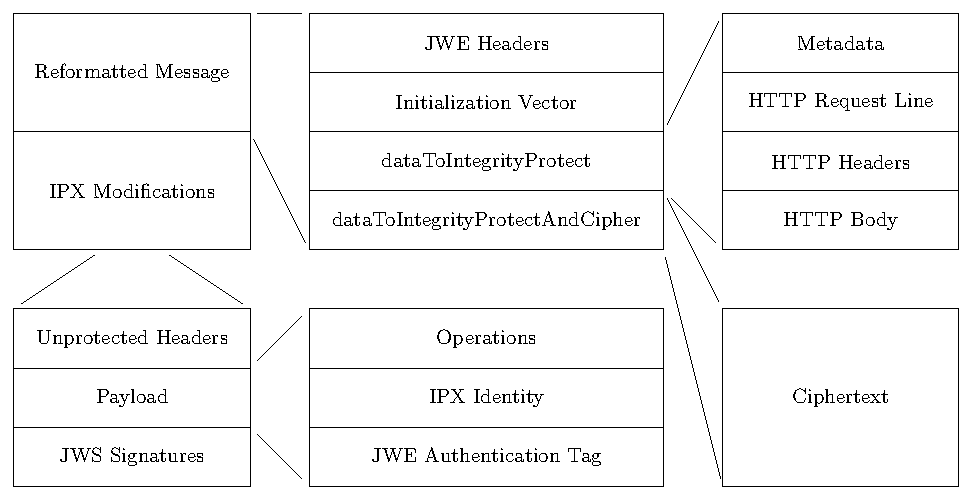
\includegraphics{n32f-message.pdf}
    \caption{N32-f message structure according to TS 29.573 (\cite{3gpp.29.573}, p. 22)}
    \label{fig:n32f-message}
\end{figure}

\end{appendices}

\end{document}
